\begin{frame}{Grafo de Fluxo de Controle}
    \begin{itemize}
        \item O grafo de fluxo de controle (do inglês, \textit{Control Flow Graph}, ou CFG) é uma IR gráfica fundamentada no controle e análise de fluxo de dados.
    
        \item Modelado como um grafo dirigido $G=(N,E)$, o CFG representa, respectivamente, blocos de código básicos $n$, de forma que $n \in N$, e a transferência de controles de um bloco a outro, modelado como uma aresta $e$, tal que $e \in E$ \cite{allen1970control}.
    \end{itemize}
\end{frame}

\begin{frame}{GFG - Exemplos}
    \begin{figure}
        \centering
        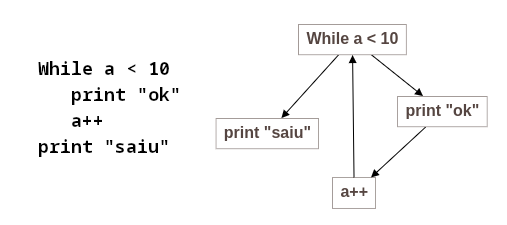
\includegraphics[width=.8\textwidth]{Figuras/cfg.png}
        \caption{Modelagem de \textit{While Statement} em CFG}
        \label{fig:enter-label}
    \end{figure}
\end{frame}

\begin{frame}{GFG - Exemplos}
    \begin{figure}
        \centering
        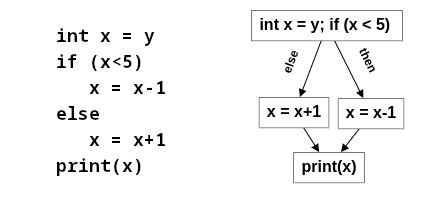
\includegraphics[width=.8\textwidth]{Figuras/cfg2.png}
        \caption{Modelagem de \textit{If Statement} em CFG}
        \label{fig:enter-label}
    \end{figure}
\end{frame}